\documentclass[12pt]{article}

\usepackage[utf8]{inputenc}
\usepackage[top=2cm]{geometry}
\usepackage{graphicx}
\usepackage{subcaption}
\graphicspath{{img}}


\title{Moogle!}
\author{Ramón Hernández Camacho}
\begin{document}

\begin{center}

    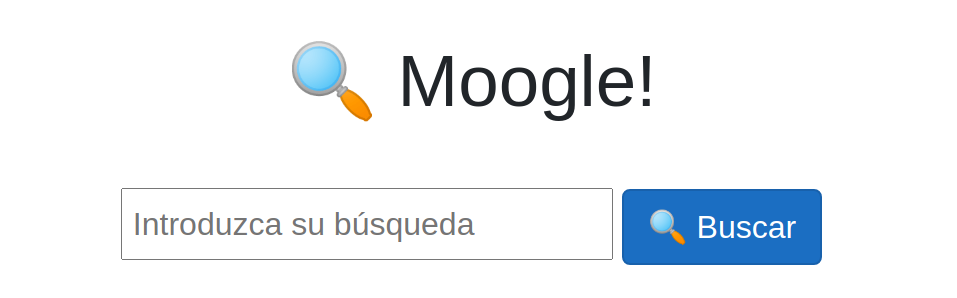
\includegraphics[width=14cm]{moogle.png}

\end{center}
Moogle! es una aplicación Web creada con el objetivo de buscar un texto determinado
en un conjunto de documentos de acuerdo a la relevancia que tiene el conjunto de
palabras introducidas por el usuario (Query) en cada documento.

Para poder cuantificar la relevancia de cada documento se ha utilizado la medida de
recuperación de información TF-IDF que traducido al español significa (Frecuencia de
Término- Frecuencia Inversa de Documento) y la fórmula del coseno.
A continuación pasaremos a describir el proceso que ocurre desde que se inicia el
proyecto hasta que se devuelven los resultados.
Todo inicia en MoogleServer quien llamará a nuestra función de la clase Moogle :
CreateCorpus dando inicio a la creación de nuestro cuerpo de documentos. Se revisa
la carpeta Content en busca de documentos TXT y por cada uno de ellos se creará un
objeto de la clase Document para un mejor manejo de la información individual. Aquí se
divide cada texto en palabras y luego se almacena en un diccionario las distintas
palabras y el número de veces que aparecen. Seguido a esto se calcula el tf idf de
cada palabra en cada documento y así quedaría confeccionado nuestro cuerpo de
documentos que al solo tener que calcularlo 1 vez cuando iniciamos el programa nos
brindará una velocidad mayor en cada búsqueda.
Al introducir el usuario una búsqueda se creara un nuevo Document con la Query al
cual también calcularemos su Tf-Idf. Terminado esto pasamos al paso de mayor
importancia el cual es el cálculo y asignación de la relevancia de cada documento a
través de la función CosRelevancia la cual usando la fórmula que se adjunta ,deter
cuan pequeño es el ángulo que determina cada vector(documento) y la query ,
mientras menor sea mayor será la relevancia.
(Ver Anexos)
Luego ordenan los documentos en dependencia de su relevancia en la función Biggest
y se le asigna a cada resultado el título del documento , una porción de su texto
llamada snippet la cual obtenemos al buscar la porción de texto de 20 palabras o
menos que contenga mayor cantidad de palabras de nuestra búsqueda, y su
relevancia. Se convierten estos valores en SearchItem y son imprimidos en pantalla
para el análisis del usuario.

\section*{Implementaciones extra:}

-Recomendación: esta solo se hará visible si nuestra búsqueda arroja menos de 3
resultados y lo que hará es llamar a la función Recomendation que recorrerá cada
palabra de la query buscando si existe en algún documento una palabra que la
contenga y esté en más de 3 documentos , en caso de no existir se toma una parte de
la palabra hasta que puedan devolverse alguna recomendación.

-Operadores \! y \^ : cada vez que se realice una búsqueda nuestro programa revisara la
existencia de ellos en nuestra query en caso de existir la palabra modificada no puede
existir en nuestro documento o su relevancia se hará 0 para el operador ! y debe existir
en nuestro documento o su relevancia se hará 0 para el operador \^ .

-Operador * : cada búsqueda que se realice se comprobara si hay presencia de este
operador , en caso positivo se cuenta la cantidad de ellos y se busca en cada
documento que existe esta palabra el Tf-Idf de la palabra para multiplicarlo por la
cantidad de operadores + 1 y cuando se termine el cálculo de la relevancia se
devuelve nuestro TF – IDF a la normalidad.

-Operador ~: se revisa en cada documento en el que existan las 2 palabras entre las
que está nuestro operador . Se recorre cada palabra de nuestro texto y voy
comparando la posición de aparición de cada palabra de la búsqueda con la última
posición que tenia de la otra palabra pues la menor distancia entre una palabra y otra
solo puede ser en las ocurrencias de la otra que la encierran . Ejemplo supongamos
que mi palabra A aparece en la posición 2 ,7 y 10 y la B en 1 y 5 la palabra B en su
aparición en la posición en 5 solo puede estar más cerca de la aparición en la pos 2 o 7
de la palabra 1 (en este caso es 7).

-Para la comodidad del usuario este puede hacer click sobre su sugerencia para que
automáticamente se realice una búsqueda basada en la recomendación dada sin
necesidad que este escriba pues este podría volver a equivocarse.
Para mayor velocidad en la búsqueda no es necesario dar click en el botón de
búsqueda sino que al presionar la tecla “enter” se realizará la búsqueda.

\newpage

\section*{Anexos}
\begin{figure}[h]
    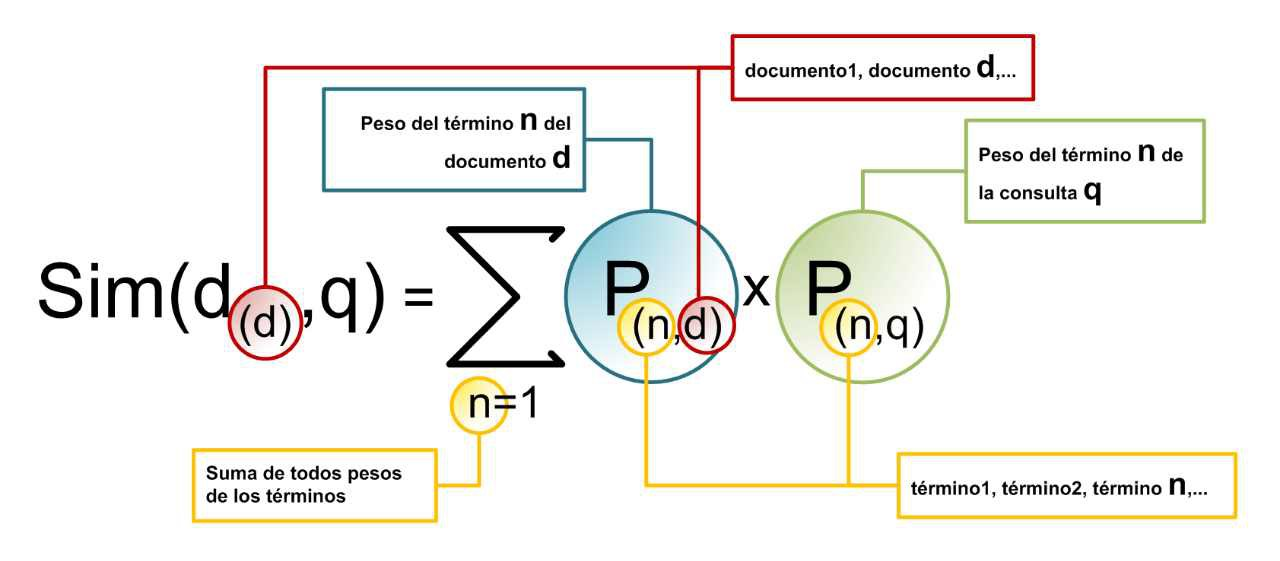
\includegraphics[width=15cm]{1.jpg}
    \caption{Formula que representa como calcular la similitud entre 1 documento y la
        query solo teniendo en cuenta el TF-IDF.}
\end{figure}


\begin{figure}[h]
    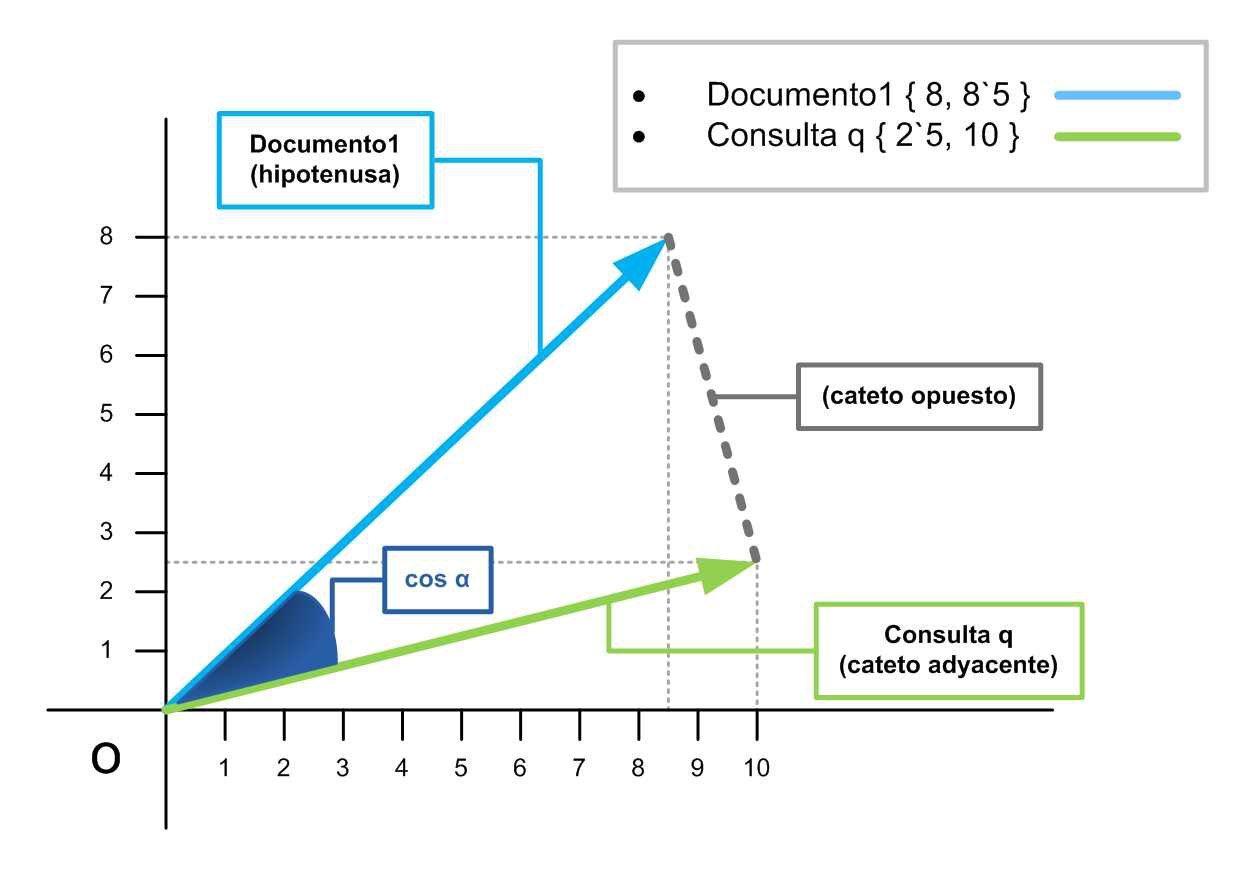
\includegraphics[width=10cm]{2.jpg}
    \caption{Representación gráfica de la similitud por coseno}
\end{figure}
\begin{equation}
    SimCos(d_{(d),q})=\frac{\sum_{n = 1}^{}(P_{( n,d) } * P_{( n,q) })   }{\sqrt[]{\sum_{n = 1}(P_{(n,d)})^2 * \sum_{n=1}(P_{(n,q)})^2}  }
\end{equation}
Figure 3: Fórmula para calcular la similitud por coseno entre 1 documento y la query


\end{document}
